\chapter{System Integration Testing and Results}

In order to validate our final product, we designed a series of tests to determine to what extent we met the hard engineering requirements outlined in our engineering requirement flowdown (Appendix \ref{App:DesignRequirements}). 

\section{Range Requirement Testing}
Being able to operate the vehicle at a distance was a very important requirement.  We wanted to verify that the remote operator console could maintain good contact with the vehicle at range and also that the router on the back of the rover gave us enough range to be able to operate the User Interface at a range as well.

We knew that the router on the back of the vehicle that powers our WiFi network that allows us to run the User Interface was going to have a shorter range than the system powering the communication with the remote operator console.  We set our requirement threshold to a range that we considered feasible based on the specifications of the router.  Our requirement was that the WiFi network and remote operator console have a range of 150 meters.

To test this, we left the vehicle and one member of our team in a stationary location and loaded the remote operator console and a laptop into another vehicle and drove as far away as possible before we lost connection.  We would stop along the way, while remaining in line of sight with the vehicle, and would send commands to the vehicle via the remote operator console.  If our team member with the vehicle saw the event happen, we knew the remote operator console still had contact.  For the WiFi network, the web-based user interface will display a message when it loses connection, so we monitored the user interface and marked when that message appeared.  

For the WiFi network, we lost connection at about 250 meters away from the vehicle.  The remote operator console still had good connection, so we kept driving.  We reached the edge of the property we were testing at about one kilometer away from the vehicle and were still able to send commands.  We know that the remote operator console as a range in excess of one kilometer, which greatly surpasses our 150 meter requirement.

\begin{table}[ht]
    \centering
    \begin{tabular}{ l | c | r }
      Verification & Requirement (meters) & Result (meters) \\ \hline
      Remote Operator Console & 150 & 1000 \\
      WiFi Network & 150 & 250 \\
    \end{tabular}
    \caption{Range requirements and verification results}
    \label{table:range_verification}
\end{table}

\section{Latency Requirement Verification}
Latency is important to be able to operate the vehicle effectively.  We do not want operators to be making decisions based on stale data, and if the video feeds are not coming through fast enough, it will make it very hard to drive the vehicle.

\begin{figure}[H]
\centerline{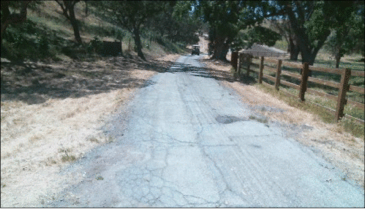
\includegraphics[angle=0, width=.5\linewidth]{front_camera_latency}}
\caption[]{Screenshot from the front facing camera on the vehicle taken during our testing}
\label{fig:front_camera_latency}
\end{figure}

There were several areas of latency that we wanted to test.  First, we wanted to test the latency from the cameras to the onboard laptop.  Second, we wanted to test the latency from the cameras to the web-based user interface and see what the difference is between the two.  Finally, we wanted to check what the latency was for vehicle state data, such as wheel speed and the readings from environmental sensing packages, from the vehicle to the user interface.  In all of these cases, we set the requirement that this latency be less than one second.

\begin{table}[ht]
    \centering
    \begin{tabular}{ l | c | r }
      Verification & Requirement (seconds) & Result (seconds) \\ \hline
      Cameras to onboard laptop & 1 & .75 \\
      Cameras to user interface & 1 & .8 \\
      Vehicle state data to user interface & 1 & 2 \\
    \end{tabular}
    \caption{Latency requirements and verification results}
    \label{table:latency_verification}
\end{table}

As shown in table \ref{table:latency_verification}, the camera feeds in both cases had a latency under our one second requirement.  The vehicle state data however, had a latency of two seconds.  We later discovered that this was due to lack of optimization.  There were points in the data pipeline that were causing data to take longer to send and be processed than we originally thought.  Displaying the data in graph form, such as the gauges for the different gas readings, added extra time to processing the data.

Future optimizations could be done to increase the speed of this processing.

\section{GPS Testing}
%Pat
\begin{figure}[H]
	\centerline{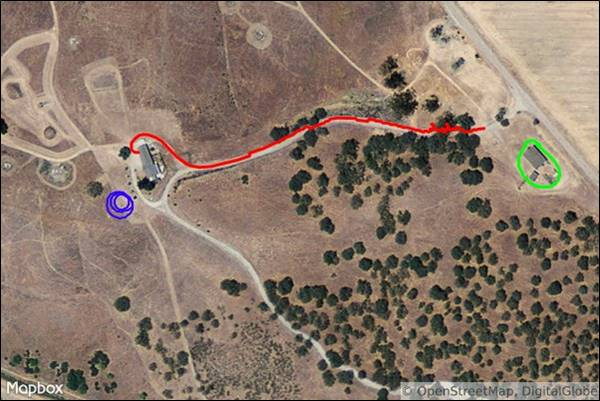
\includegraphics[angle=0, width=.8\linewidth]{GPS_MAP}}
	\caption[]{Logged GPS tracks of various field testing activities}
	\label{fig:GPSMAP}
\end{figure}

\section{Localization and Mapping Testing}
%Pat

\begin{figure}[H]
	\centering
	\begin{subfigure}{.5\textwidth}
		\centering
		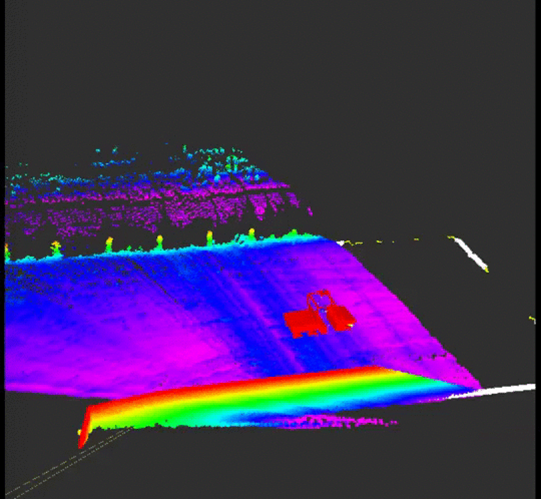
\includegraphics[width=.8\linewidth]{3dviz1}
%		\caption{Front Mounted Static LIDAR}
		\label{fig:3dviz1}
	\end{subfigure}%
	\begin{subfigure}{.5\textwidth}
		\centering
		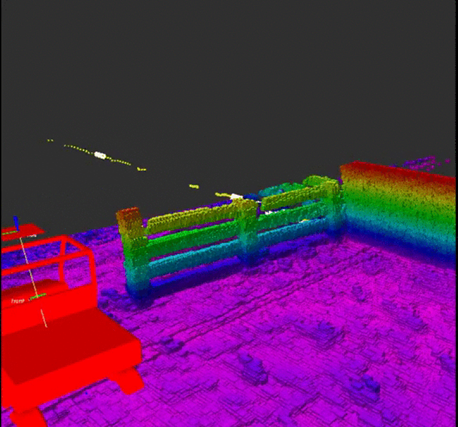
\includegraphics[width=.8\linewidth]{3dviz2}
%		\caption{Roll Cage Mounted Sweeping LIDAR}
		\label{fig:3dviz2}
	\end{subfigure}
	\caption{3D visualization of vehicle during mapping activity}
	\label{fig:3dviz}
\end{figure}


\section{Environmental Sensor Package Testing}
Our environmental sensing packages are a critical component of our vehicle.  To test the effectiveness of these packages, we set a small, controlled burn and circled the fire with our vehicle.  With each pass around the fire we increased the radius of our lap.  The point of this was to test our ability to pinpoint the location of a fire using a the mapping and localization system in conjunction with the environmental sensing packages.

\begin{figure}[H]
\centerline{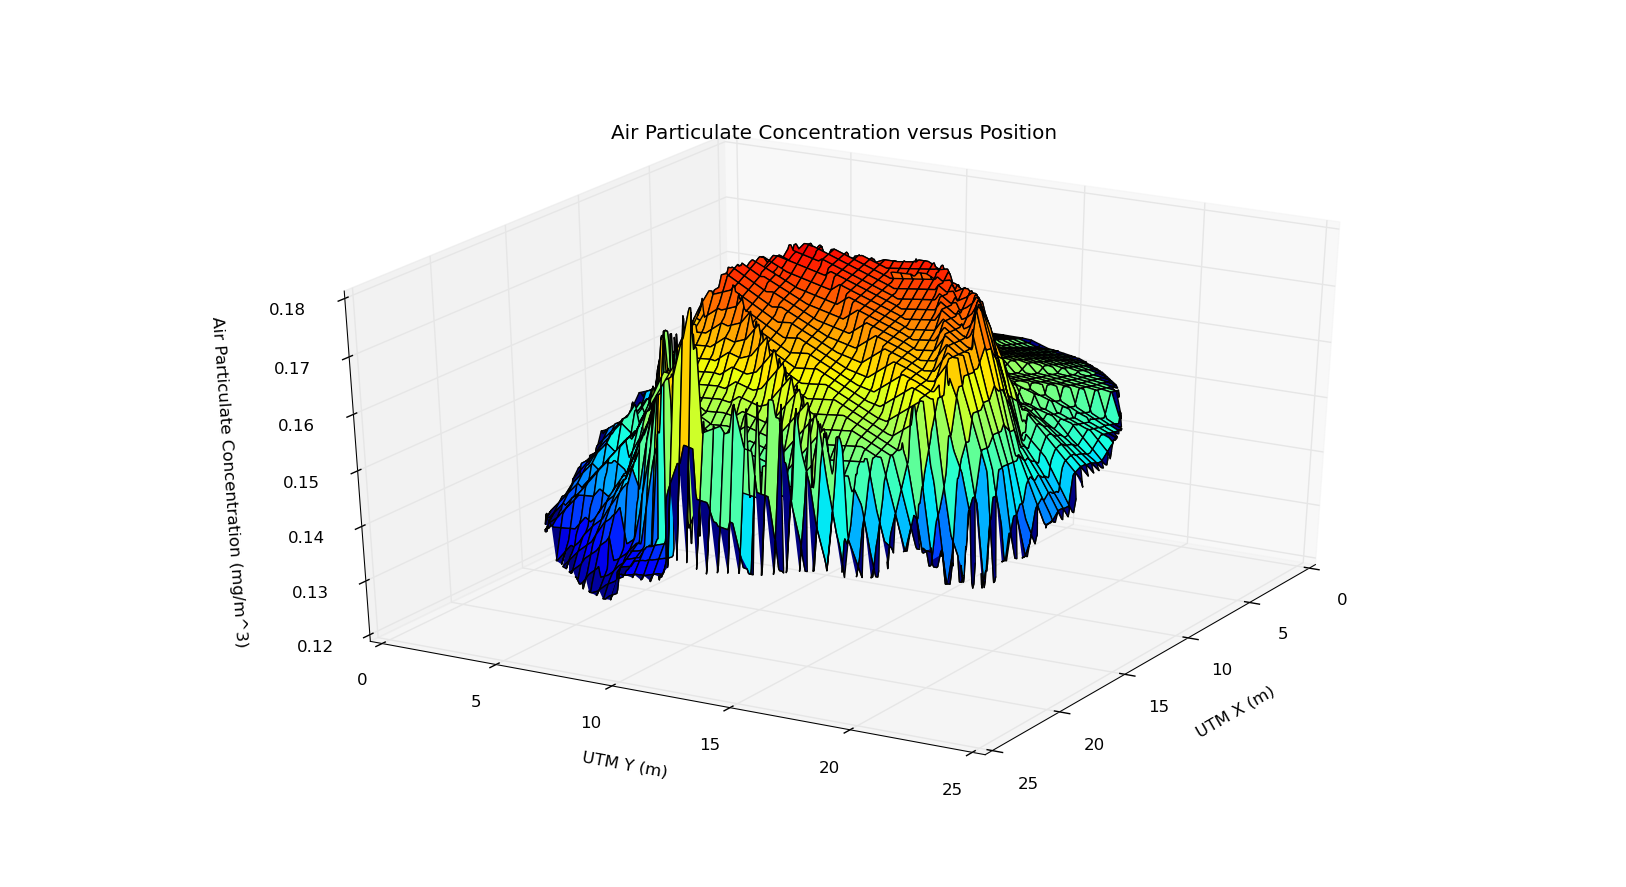
\includegraphics[angle=0, width=1\linewidth]{air_particulare_versus_position_graph.png}}
\caption[]{The results of our controlled burn test.}
\label{fig:air_particulate_versus_position_graph}
\end{figure}

As shown in figure \ref{fig:air_particulate_versus_position_graph} our environmental sensing units are able to detect the presence of environmental hazards.  The x and y-axes are position, and the z-axis is the concentration of air particulates, which in this case is the presence of smoke.  The concentration peaks at the center of the graph and decreases as position away from the center increases.  These are the expected results, since the concentration of smoke should decrease as we move away from the fire.

We can also see how the different sensor packages detect the gases differently.  While not an actual requirement, we were curious to see how the different sensor packages functioned.  The point to having redundant sensors was to be able to continue detecting environmental hazards even if one package dies.  We wanted to know if the packages behave comparably to each other.


\begin{figure}[H]
\centerline{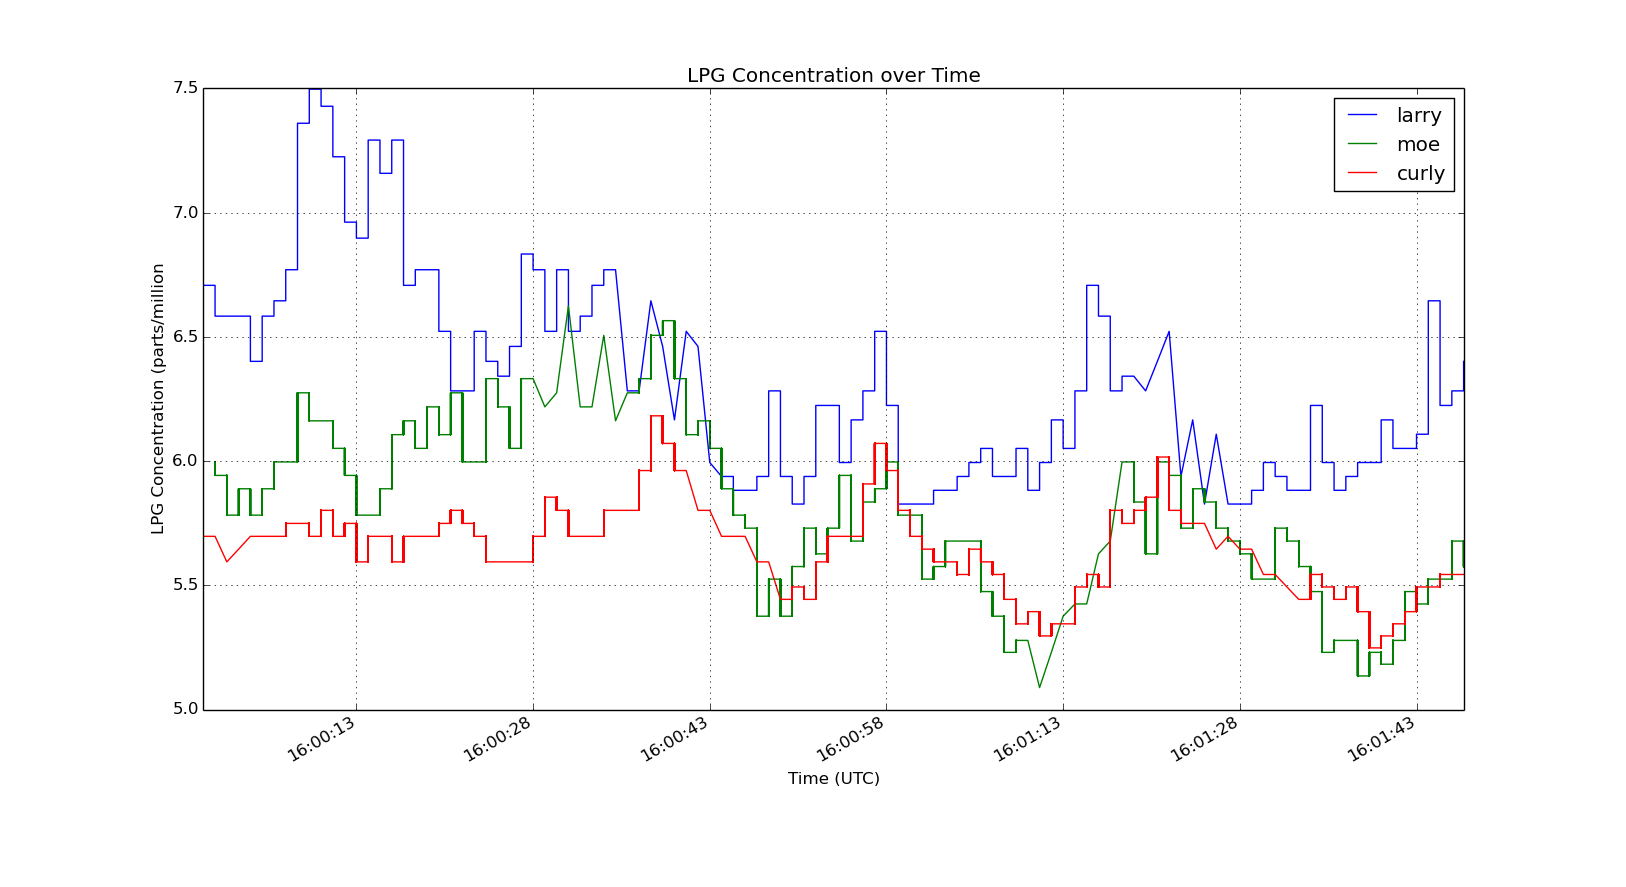
\includegraphics[angle=0, width=1\linewidth]{allSensor_lpg_versus_time_graph}}
\caption[]{The resulting web from attaching string to each camera and then tying those strings to posts and placing them in the ground when the post left the field of view of the respective camera.}
\label{fig:allSensor_lpg_versus_time_graph}
\end{figure}

Figure \ref{fig:allSensor_lpg_versus_time_graph} shows the measurement of LPG versus time for each of the environmental sensing units.  While all of the sensing units follow a similar trend, each one displays different levels of LPG.  When the test started, we were closest to the fire, which is why the LPG concentration is the higher at the beginning of the plot.  Each sensor is also positioned in different places on the vehicle which explains some of the differences.  However, all of the sensors show an increase in LPG closest to the fire, and less LPG as the vehicle moved away from it, which was what we expected.

\section{Blind-spot Testing}
To test the blind-spots on the vehicle, we attached string to the cameras and placed posts in the ground when they had just left the field of view of the cameras.  The strings were all of close to equal length such that we could measure the distance between the posts in a straight line.  We can then convert those distances into angles that define the field of view of the vehicle, and the size of the blind-spots of the vehicle.

\begin{figure}[H]
\centerline{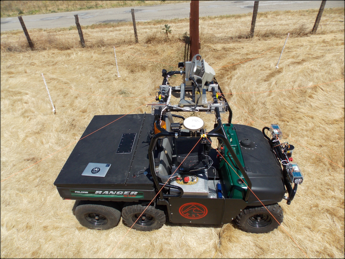
\includegraphics[angle=0, width=.5\linewidth]{blindspot_verification}}
\caption[]{The resulting web from attaching string to each camera and then tying those strings to posts and placing them in the ground when the post left the field of view of the respective camera.}
\label{fig:blindspot_verification}
\end{figure}

Our requirement was that the cameras would offer 360 degrees of view.  In other words, our requirement was to have no blind-spots.  Unfortunately, based on the resulting calculations from the measurements we took, each camera only provided 65 degrees of coverage, resulting in a total 260 degrees of view.  Each blind-spot between the cameras was only 25 degrees, but this still fell short of our requirement.

\begin{figure}[H]
\centerline{\includegraphics[angle=0, width=.5\linewidth]{Blindspots_measurement}}
\caption[]{The distance between the posts and the angles we derived between them.}
\label{fig:blindspot_measurement}
\end{figure}

We could further increase our field of view though by adding two more cameras to the vehicle.  and placing them on the side of the roll cage angled backwards.  We would then take the two cameras already on the roll cage and angle them more forwards.  These four cameras together would then cover the current blind-spots on the vehicle.